% Where Does Federal Equalization Money Go? Spending, School Inputs and Learning under Brazil's Fundeb VAAT
% Working paper, November 2026 -- version formatted for Education Finance and Policy
\documentclass[12pt,letterpaper]{article}
\usepackage{fontspec}
\setmainfont{TeX Gyre Termes}
\usepackage[english]{babel}
\usepackage[letterpaper,margin=1in]{geometry}
\usepackage{setspace}
\doublespacing
\usepackage{microtype}
\usepackage{amsmath,amssymb}
\usepackage{booktabs,array}
\usepackage{graphicx}
\usepackage{adjustbox}
\usepackage{enumitem}
\usepackage{caption}
\usepackage{float}
\usepackage[document]{ragged2e}
\usepackage[nolists]{endfloat}
\captionsetup{font=small,labelfont=bf}
\usepackage[round]{natbib}
\usepackage{xcolor}
\usepackage[colorlinks=true,linkcolor=black,citecolor=black,urlcolor=blue!50!black]{hyperref}
\usepackage{xurl}
\newcommand{\todo}[1]{\par\noindent\colorbox{yellow!25}{\parbox{\dimexpr\linewidth-2\fboxsep}{\small\textbf{TO DO:} #1}}\par}
\newcommand{\reais}{R\$}
\graphicspath{{figuras/}}
\setlist{itemsep=2pt,topsep=4pt}

\title{\textbf{Where Does Federal Equalization Money Go?}\\[0.2em]\large Spending, School Inputs and Learning under Brazil's Fundeb VAAT}
\author{Caio A. F. Cunha\\[0.2em]\normalsize Independent researcher, Brazil\thanks{ORCID: \href{https://orcid.org/0009-0008-2153-901X}{0009-0008-2153-901X}. Data, code and replication instructions: \url{https://github.com/Caioalexnes/Brazilian-Basic-Education-Analysis}. The pre-analysis plan was deposited before any outcome was related to the treatment: \url{https://doi.org/10.5281/zenodo.24391650}.}}
\date{November 2026}

\setlength{\emergencystretch}{2em}
\begin{document}
\maketitle

\begin{abstract}
\singlespacing
\noindent Since 2021, Brazil's federal government tops up the education resources of every public school network whose resources per weighted student fall below a national minimum. By 2025 this complementation, the VAAT of the Fundeb, paid \reais{}~24.5 billion to 2,372 municipal networks. Following a pre-registered plan, I measure exposure by the amount the legal formula predicts from 2019 fiscal data and compare networks within states. The money reached the networks with the lowest spending and the poorest students, but their enrollment was already growing faster before 2019, partly because state schools were moving to them. The pre-registered estimate for spending per student is positive but driven by that growth, which lowered spending per student in the formula's base year. Total spending, with no differential trend before 2019, rose by about twice the VAAT money received; the rest matches transfers from the state-level Fundeb, which follow enrollment and rose from 2020, before any VAAT payment. Learning did not change detectably: at the 75th percentile of exposure, the 95\% intervals exclude effects above 0.050 student standard deviations in the 5th grade and 0.055 in the 9th, and in the 5th grade the estimate continues a trend that predates the program.

\medskip
\noindent\textbf{Keywords:} school finance; intergovernmental transfers; Fundeb; continuous difference-in-differences; pre-analysis plan; Brazil.\\
\noindent\textbf{JEL codes:} H75; H77; I22; I28.\\
\noindent\textbf{Funding:} The author received no financial support for the research reported in this paper.
\end{abstract}

\newpage
\section{Introduction}

Equalization transfers are the main tool that federations use to make the resources of local school systems less unequal. Brazil made such a transfer much larger in 2020. Constitutional Amendment 108 and Law 14.113 kept the Fundeb, the system of state-level funds that pools most education revenues, and added a federal complementation paid to individual school networks: the VAAT. Every network whose total resources per weighted student fall below a national minimum is topped up exactly to that minimum. The VAAT paid \reais{}~3.8 billion in 2021 and \reais{}~24.5 billion in 2025, to 2,372 of the country's 5,570 municipal networks (Figure~\ref{fig:anos}), and its share of the Fundeb keeps growing until 2026.

This paper asks where that money went and what it did to spending, school inputs and learning in the municipal networks. The question has a simple version, whether the transfer raised spending and test scores, and a harder one, whether the design of the transfer allows us to tell. I answer both following a pre-analysis plan deposited before any outcome was related to the treatment \citep{cunha2026pap}, amended once before the analysis \citep{cunha2026add}. Each network's exposure, the dose, is the complementation that the legal formula predicts from fiscal data of 2019, summed over 2021 to 2025. Because the formula only converts differences in 2019 fiscal capacity into reais, the design compares networks of the same state with more and less fiscal capacity, and its credibility rests on whether their outcomes would have evolved in parallel without the VAAT. The plan therefore pairs the main estimate, a long difference with a continuous dose, with an event study, a comparison between the municipal and the state network of the same municipality, and a regression kink at the 2021 threshold.

There are three findings. First, the money went where the formula says it should: to the networks with the least resources per student, which are also the poorest and are concentrated in the Northeast. In 2019, networks in the top tercile of the dose spent \reais{}~7,391 per student at 2025 prices, against \reais{}~13,448 in networks with no dose (Table~\ref{tab:descritivas}). They were also on a different path. Within states, their enrollment grew faster before 2019, by 2.2 log points per \reais{}~1,000 of dose between 2015 and 2019, partly because state schools were being handed over to the municipalities.

Second, spending rose, but the design cannot attribute it to the VAAT alone. The pre-registered estimate is \reais{}~133 of additional spending per student for each \reais{}~1,000 of dose. But spending per student had been falling in these networks relative to others until 2019, because their enrollment was growing; the base year of the formula is the bottom of that decline, and measured from earlier years the estimate is zero. Total spending tells a cleaner story: it has no differential trend before 2019 and rises from 2020 on. By 2025 the increase is about twice the VAAT money that these networks actually received, which was much less than the formula predicted from 2019 data. The rest matches higher transfers from the state-level Fundeb, which are distributed by enrollment and began rising in 2020, before any VAAT payment. The regression kink, which the plan expected to have little power, is uninformative.

Third, learning did not change detectably. At the 75th percentile of the dose, the pre-registered estimates are 0.022 student standard deviations in the 5th grade and in the 9th, with 95\% intervals that exclude effects above 0.050 and 0.055. These point estimates are close to the 0.018 that the plan expected if Brazilian schools turned money into learning at the rate estimated for the United States \citep{jackson2024}, but that expectation assumed the money the formula predicts, about twice the money that arrived, and the design cannot distinguish the estimates from zero. In the 5th grade the estimate is the continuation of a trend that began a decade before the program; net of that trend it is 0.007. The comparison within municipalities, which absorbs local shocks, is close to zero in both grades.

The paper contributes in four ways. It is the first evaluation of the VAAT complementation that uses its formula to measure exposure and that studies spending and learning together; Section~\ref{sec:literatura} discusses the two earlier studies of the reform. Second, it documents a problem that any evaluation of a per-student formula faces: a capacity measure divided by enrollment in a base year selects networks whose enrollment is growing, so comparisons of spending per student anchored in that year mix the transfer with the denominator. Third, it bounds the learning effect of a large equalization transfer in a middle-income country, adding to a literature built mostly on reforms in the United States \citep{jackson2016,lafortune2018,jackson2024} and on earlier Brazilian transfers \citep{menezes2007,litschig2013}. Fourth, every analytical choice was registered before the corresponding outcome was seen, and every departure from the plan, including two of my own errors, is reported in Appendix~\ref{app:desvios}.

\section{The VAAT complementation}\label{sec:politica}

The Fundeb is a set of 27 state-level funds. Each pools most of the education revenues of a state and its municipalities and redistributes them among the state network and the municipal networks of that state in proportion to enrollment, with weights by stage and modality. Before 2021 the federal government added only one complementation, now called the VAAF, to the funds of the states where resources per student were lowest. Constitutional Amendment 108/2020 made the Fundeb permanent and created two new federal complementations, both paid to individual networks: the VAAT, studied here, and the VAAR, which rewards learning results and is paid from 2023.

For each network, the VAAT is the ratio of all resources earmarked for education, including Fundeb receipts and other earmarked revenues, to weighted enrollment (Law 14.113, art.~13, \S3). The revenues are those of the second year before the year of reference (art.~15), so the VAAT of 2021 uses 2019 revenues, and the weights of early childhood education are multiplied by 1.5 (art.~43). Each network below the national minimum, the VAAT-MIN, is topped up exactly to that minimum, provided it submitted its fiscal data on time (art.~13, \S4). Half of the total VAAT complementation must go to early childhood education, distributed among networks by an indicator, the IEI (art.~28); at least 15\% must go to capital spending (art.~27); and the money counts toward the rule that at least 70\% of Fundeb resources pay education professionals (art.~26). The VAAT share of the Fundeb grows from 2\% in 2021 to 10.5\% in 2026 \citep{tanno2021}.

The VAAT-MIN rose from \reais{}~4,846 per weighted student in 2021 to \reais{}~8,021 in 2025, and the number of recipient municipal networks from 1,527 to 2,372 (Figure~\ref{fig:anos}). The 2021 money was small and paid from July 2021 to January 2022. The same reform made learning high-stakes for municipalities through the VAAR and through the requirement that every state distribute part of the municipal share of the ICMS according to learning outcomes.

\begin{figure}[!htbp]
\centering
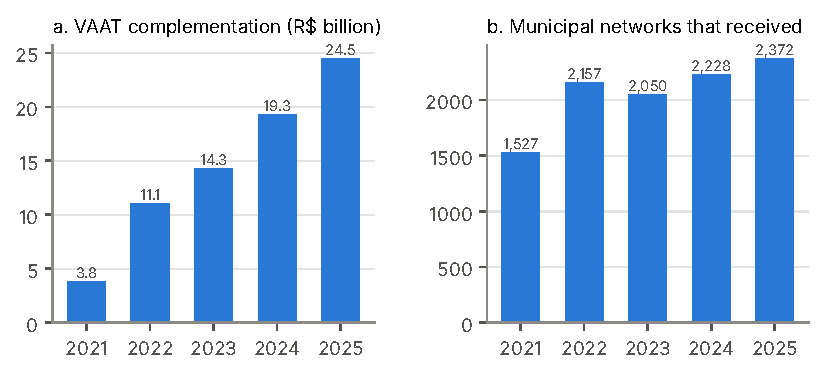
\includegraphics[width=0.9\linewidth]{f1_vaat_anos.pdf}
\caption{VAAT complementation by year. Annex III of the final December portaria of each year; nominal values. In 2025, one state network also received.}\label{fig:anos}
\end{figure}

\section{Related literature}\label{sec:literatura}

Whether a grant to a local government raises spending by the amount of the grant is an old question. Grants tend to raise local spending by more than equal increases in local income, the flypaper effect \citep{hines1995}, but how much of a grant meant for schools ends up in schools depends on how local governments adjust their own revenues. \citet{gordon2004} finds that Title I grants to U.S. school districts were not offset at first, but that local governments crowded out the changes in the grants within about three years. In Brazil, \citet{litschig2013} use the population thresholds of the municipal revenue-sharing fund (FPM) and find that extra transfers raised local government spending per capita by about 20 percent over four years, with no sign of crowding out of own or other revenues, and raised schooling and literacy. The VAAT differs from these grants in that it is earmarked for education, is paid to individual school networks, and tops each of them up exactly to a minimum, so that its amount is a known function of the network's own earlier revenues and enrollment. Section~\ref{sec:fontes} shows that this last feature makes pass-through hard to measure.

Evidence that school spending raises learning and attainment comes mostly from the United States. \citet{jackson2016} find that increases in spending per student induced by court-ordered school finance reforms raised educational attainment and adult earnings, more so for children from low-income families, and \citet{lafortune2018} find that the reforms after 1990 raised spending sharply in low-income districts and student achievement gradually in the following years. Summarizing U.S. evaluations, \citet{jackson2024} estimate that \$1,000 more per pupil for four years raises test scores by 0.0316 standard deviations, the benchmark the plan used to set the expected effect of the VAAT.

Brazil's earlier funding reform, the Fundef of 1998, first pooled education revenues within each state and redistributed them by enrollment. \citet{menezes2007} find that it raised the relative wages of public school teachers and the relative proficiency of public school students, and present evidence that part of the gain in proficiency is related to the higher wages. \citet{estevan2015} finds that the increases in public education spending it caused reduced the share of private school enrollment in the first grade, with smaller effects in later grades. \citet{cruz2018} relate the net transfers of the Fundef and the Fundeb received while children were of school age to their outcomes in the censuses of 2000 and 2010, and find small increases in school attendance and reductions in age-grade distortion, larger for children of lower socioeconomic status, and effects on child labor close to zero.

Two studies evaluate the reform of 2020. \citet{franca2026} estimate the effect of the VAAT on the supply of early childhood education with a staggered difference-in-differences that compares recipients with never-recipients near the 2021 threshold; they do not study spending or learning, and several of their outcomes show differential trends before treatment. \citet{lima2025fundeb} classify municipalities by their net balance in the Fundeb redistribution, simulated for 2021 with the shares of 2019, and find that the largest winners improved early-grade Portuguese scores and the Ideb, with no effect in the late grades. Their treatment is a municipality's position in a redistribution that predates the reform, so it does not isolate what the reform changed.

This paper isolates the VAAT, whose amount follows a formula applied to data measured before the program, and uses that formula to measure exposure instead of a binary treatment. It studies spending, school inputs and learning in the same networks, so the learning estimates can be read against the money that arrived. And it shows that a transfer that divides a base-year capacity by base-year enrollment selects networks whose enrollment is changing, which complicates any comparison of spending per student and ties the transfer to other revenues that follow enrollment.

\section{Data and sample}\label{sec:dados}

The treatment data come from the official lists of each year. The VAAT of 2021 of the 5,234 networks habilitated by mid-2021 (5,208 municipal and 26 state networks) is reproduced, with each network's revenues and weighted enrollment, in the annex of \citet{tanno2021}; for the 1,422 recipients that also appear in the official December list it matches to within 0.024\%. The December portarias of 2021 to 2025 give the recipients, the amount per weighted student and the IEI share of each year, and the later adjustments for 2023 and 2024 are used in a robustness check.

Spending is committed spending in function 12 (education) of the municipal accounts \citep[Siconfi, DCA, Annex I-E; definition of][]{cunha2026a}, divided by the enrollment of the municipal network plus the early childhood enrollment of private schools under agreement with the municipality, at 2025 prices. School inputs and enrollment by network come from the Censo Escolar and from Inep's educational indicators. For an exploratory decomposition of spending, revenues come from Annex I-C of the same accounts. Learning outcomes are Inep's Ideb files by municipality and network, which give for every round from 2005 to 2025 the Saeb mean scores in mathematics and Portuguese, their standardized mean $N$ on a scale from 0 to 10, the flow indicator $P$ and the Ideb. One point of $N$ equals 0.507 student standard deviations in the 5th grade and 0.574 in the 9th (Appendix~\ref{app:dados}).

The main sample is the 5,208 municipal networks of the mid-2021 list. The 105 networks habilitated later enter only in a robustness check, because late habilitation may respond to the expected gain. A network enters a long difference if the outcome is observed in both years: 5,145 networks for spending, 4,768 for the 5th-grade $N$ and 2,726 for the 9th-grade $N$, which is observed only where the municipal network has enough students in the late grades.

\section{Design}\label{sec:desenho}

\subsection{The dose}

Let $x_i = \text{VAAT}_{i,2021}/4{,}846.26 - 1$ be the position of network $i$ relative to the 2021 threshold. For each year $t$ from 2021 to 2025, the predicted complementation is
\begin{equation}
\hat Z_{it} = \max\left(0,\ \text{VAAT-MIN}_t - g_t \cdot \text{VAAT}_{i,2021}\right),
\end{equation}
where $g_t$ is set so that the number of sample networks with $\hat Z_{it}>0$ equals the number that actually received in year $t$. The dose $D_i = \sum_t \hat Z_{it}$ is in thousand reais of 2025 per weighted student. It depends only on data of 2019 and on one aggregate number per year, whereas the money actually received depends on later enrollment, which the VAAT itself affects. 59.0\% of the networks have $D_i=0$; among the others the median is 2.99, the 75th percentile 5.01 and the 90th percentile 6.65. Figure~\ref{fig:dose} shows the dose as a function of $x_i$. The correlation between the predicted dose and the money actually received is 0.775.

\begin{figure}[!htbp]
\centering
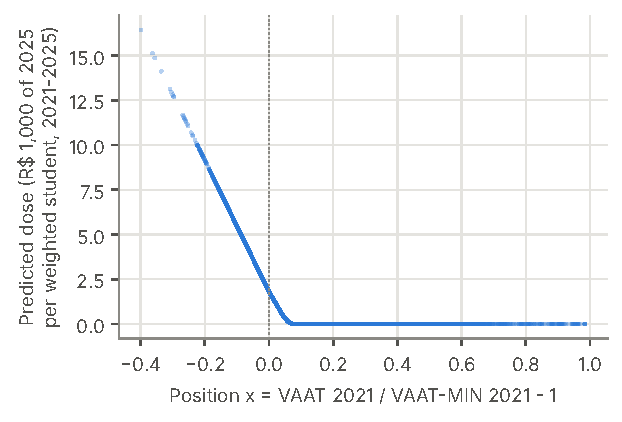
\includegraphics[width=0.55\linewidth]{f2_dose_posicao.pdf}
\caption{Predicted dose and the 2021 VAAT position. Main sample, $x\le 1$. The dose is positive for some networks above the 2021 threshold because the threshold rose faster than their VAAT in later years.}\label{fig:dose}
\end{figure}

\subsection{Estimation}

The main specification is a long difference,
\begin{equation}\label{eq:ld}
\Delta Y_i = \lambda_s + \beta D_i + \gamma' W_i + \varepsilon_i ,
\end{equation}
where $\lambda_s$ are state fixed effects, which absorb the VAAF, each state's ICMS rule and everything else common within a state, and $W_i$ holds the INSE of 2019 (the socioeconomic level of the network's students), the log of the 2020 population and the ICMS share of current revenue in 2019. Standard errors are clustered by IBGE immediate region (509 clusters). With a continuous dose, $\beta$ is an average causal response only under strong parallel trends and a linear dose response \citep{callaway2024}, so the plan gives equal prominence to $\text{ATT}^o$, the average effect on the treated relative to zero-dose networks, from a cubic B-spline in the dose estimated with the same fixed effects and covariates. The event study replaces $\Delta Y_i$ with the full panel, unit and state-by-year fixed effects and a dose coefficient for each year relative to 2019. Its pre-trend test uses a wild cluster bootstrap $p$-value \citep{cameron2008}; the plan's sensitivity analyses are the relative-magnitudes bounds of \citet{rambachan2023} and a dose-specific linear trend fitted to the coefficients from 2009 to 2017.

The within-municipality comparison uses the state network of the same municipality, which faces the same local shocks but receives no municipal VAAT:
\begin{equation}
\Delta Y^{\text{mun}}_i - \Delta Y^{\text{state}}_i = \lambda_s + \beta^{W} D_i + \gamma' W_i + \varepsilon_i ,
\end{equation}
with the change in the state network alone as a negative control. Finally, the 2021 threshold creates a kink in the 2021 money as a function of $x_i$, which I use to estimate how much of the first transfers became spending \citep{card2015,calonico2014}.

\subsection{Registration and what changed}

The plan was deposited before any outcome was related to the dose. Before the analysis, I tested every estimator on simulated outcomes built on the real treatment data. Three problems led to an addendum, deposited before any outcome was used \citep{cunha2026add}: the cluster-robust pre-trend test rejected 8.6\% of the time under the null, so its $p$-value now comes from a wild bootstrap (6.6\%); the plan's rule that a breakdown value of $\bar M$ below 1 marks results as not robust was triggered in every simulation, even with parallel trends and effects of six standard errors, so it was removed; and the plan had overstated the power of the kink. Before each stage, the details the plan left open were fixed in a dated file, and one outcome, the Saeb participation rate, had to be dropped because Inep masks the municipality code in the public school files. Appendix~\ref{app:desvios} lists every departure.

\section{Where the money went}\label{sec:onde}

Table~\ref{tab:descritivas} compares networks by dose. The formula did what it was meant to do. The higher the dose, the lower the 2019 VAAT and the 2019 spending per student, the poorer the students and the lower the test scores. Networks in the top tercile spent 45\% less per student than networks with no dose; 78\% of them are in the Northeast, against 7\%. They are also larger and more municipalized: in the top tercile the state network had only 11\% of public fundamental enrollment, against 39\% in zero-dose municipalities.

\begin{table}[!htbp]
\centering
\caption{Networks by predicted dose}\label{tab:descritivas}
\small
\begin{adjustbox}{max width=\linewidth}
\begin{tabular}{lrrrr}
\toprule
Dose group & Zero & Low & Middle & High \\
\midrule
Networks & 3{,}072 & 712 & 712 & 712 \\
VAAT 2021 (R\$ per weighted student) & 6{,}415 & 5{,}027 & 4{,}686 & 4{,}260 \\
Predicted dose (R\$ 1,000) & 0.00 & 0.74 & 3.01 & 6.24 \\
Spending per student 2019 (R\$ of 2025) & 13{,}448 & 9{,}524 & 8{,}338 & 7{,}391 \\
Municipal enrollment 2019 & 4{,}145 & 3{,}478 & 4{,}110 & 5{,}418 \\
Enrollment growth 2015-2019 (log points x 100) & 0.0 & $-$2.5 & $-$4.0 & 0.8 \\
State share of public fundamental enrollment 2019 & 0.39 & 0.26 & 0.14 & 0.11 \\
INSE 2019 & 5.02 & 4.61 & 4.38 & 4.25 \\
Population 2020 (thousands, median) & 7.9 & 14.5 & 15.5 & 19.2 \\
Northeast & 0.07 & 0.46 & 0.73 & 0.78 \\
N, 5th grade, 2019 & 6.33 & 5.89 & 5.59 & 5.53 \\
N, 9th grade, 2019 & 5.37 & 5.03 & 4.94 & 4.91 \\
\bottomrule
\end{tabular}
\end{adjustbox}
\par\smallskip\begin{minipage}{0.95\linewidth}\footnotesize Means over the 5,208 municipal networks of the main sample, unless stated. Low, middle and high are terciles of the positive predicted dose. Enrollment growth: municipal-network enrollment, Censo Escolar. N: standardized Saeb mean of the municipal network (0 to 10).\end{minipage}

\end{table}

The levels differ across states, but the design compares networks within a state, and within states the differences are about change. Figure~\ref{fig:matriculas} shows event studies of enrollment, with state-by-year fixed effects, by network. In municipalities with a higher dose, the state network was shrinking relative to others, before and after 2019: in the late grades of fundamental, state enrollment fell by 7.4 log points per \reais{}~1,000 of dose between 2015 and 2025, and municipal enrollment rose by 2.5. Students were moving from state to municipal schools. Total enrollment across all networks also grew steadily, by 1.5 to 1.7 log points per \reais{}~1,000 over the decade. All pre-trend tests reject ($p \le 0.004$).

\begin{figure}[!htbp]
\centering
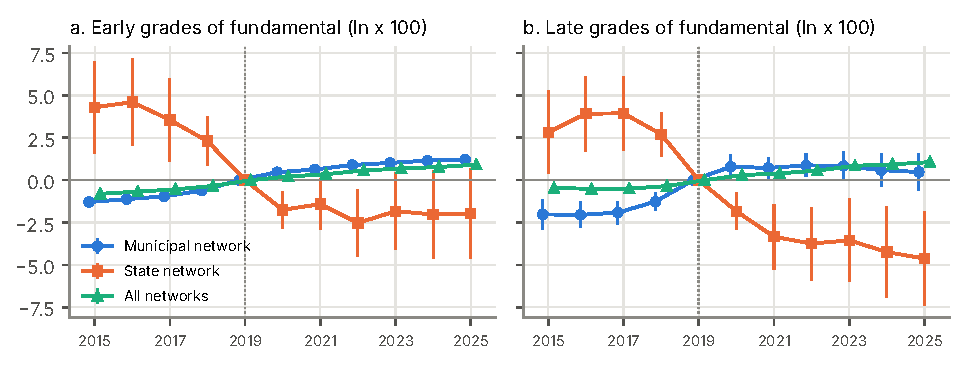
\includegraphics[width=0.95\linewidth]{f4_matriculas_redes.pdf}
\caption{Enrollment by network. Event-study coefficients of the dose on ln(1 + enrollment), $\times 100$, relative to 2019, with unit and state-by-year fixed effects and the covariates interacted with year; 95\% intervals clustered by immediate region. Exploratory, not in the plan.}\label{fig:matriculas}
\end{figure}

This matters for the design. The VAAT of 2021 divides 2019 revenues by 2019 enrollment. A network whose enrollment grew faster has, for the same revenues, a lower VAAT and a higher dose. The dose therefore selects networks that were absorbing students, and any outcome divided by enrollment, or affected by who the students are, is exposed to that selection.

\section{Spending}\label{sec:gasto}

\subsection{The pre-registered estimate}

Table~\ref{tab:gasto} reports the pre-registered results. Each \reais{}~1,000 of predicted dose is associated with \reais{}~133 more spending per student in 2025 relative to 2019 (95\% interval 90 to 176); at the 75th percentile of the dose, \reais{}~668 per student per year. Two benchmarks help to read it. The formula predicts \reais{}~281 of VAAT money per enrolled student in 2025 for each \reais{}~1,000 of dose; the money actually received was \reais{}~109, because after 2021 the networks with the highest predicted dose received less than predicted (Section~\ref{sec:fontes}). The estimate is therefore larger than the money that arrived. The estimate survives every robustness check of the plan except one: with $g_t$ taken from the growth of total Fundeb revenue, which gives a positive dose to most networks, it is $-22$ (interval $-70$ to 27).

\begin{table}[!htbp]
\centering
\caption{Spending per student (P1)}\label{tab:gasto}
\small
\begin{adjustbox}{max width=\linewidth}
\begin{tabular}{lrrcr}
\toprule
Specification & Estimate & (SE) & 95\% interval & Networks \\
\midrule
Long difference, $\beta$ & 133.3$^{***}$ & (22.0) & [90.1, 176.4] & 5{,}145 \\
ATT$^o$ & $-$117.5 & (120.7) & [$-$338.1, 132.8] & 5{,}145 \\
Mean of $h'(D)$ over the treated & 220.9 & (67.0) & [91.1, 353.5] & 5{,}145 \\
Benchmark: predicted VAAT money, 2025 & 280.6 & (2.8) & & \\
Benchmark: VAAT money received, 2025 & 108.9 & (11.2) & & \\
\midrule
(1) No covariates & 90.9$^{***}$ & (24.0) & [43.7, 138.1] & 5{,}145 \\
(3) 2019 level as covariate & 127.0$^{***}$ & (30.0) & [68.2, 185.8] & 5{,}145 \\
(4) Excluding Ceará & 127.2$^{***}$ & (22.9) & [82.2, 172.1] & 4{,}961 \\
(5) Trimming the 1\% tails of the change & 143.2$^{***}$ & (20.8) & [102.3, 184.0] & 5{,}041 \\
(6) Zero-dose networks only if $x \le 0.3$ & 137.3$^{***}$ & (22.1) & [93.9, 180.6] & 3{,}873 \\
(7a) Dose from money received & 286.0$^{***}$ & (25.6) & [235.7, 336.4] & 5{,}145 \\
(7b) $g_t$ from Fundeb revenue growth & $-$21.8 & (24.7) & [$-$70.3, 26.8] & 5{,}145 \\
(7c) Dose in nominal reais & 143.7$^{***}$ & (23.9) & [96.7, 190.7] & 5{,}145 \\
(7d) Dose per enrolled student & 105.5$^{***}$ & (17.7) & [70.8, 140.3] & 5{,}145 \\
(8) Including the 105 late recipients & 127.5$^{***}$ & (20.1) & [87.9, 167.1] & 5{,}247 \\
(9) Weighted by 2019 enrollment & 179.6$^{***}$ & (37.6) & [105.8, 253.3] & 5{,}145 \\
(10) Heteroskedasticity-robust errors & 133.3$^{***}$ & (22.5) & [89.1, 177.5] & 5{,}145 \\
\bottomrule
\end{tabular}
\end{adjustbox}
\par\smallskip\begin{minipage}{0.95\linewidth}\footnotesize Change in spending per student from 2019 to 2025, in reais of 2025, per R\$ 1,000 of cumulative predicted dose. State fixed effects; covariates INSE 2019, ln population 2020 and ICMS share 2019; errors clustered by immediate region (509 clusters). ATT$^o$ and $h'$: cubic B-spline in the dose, bootstrap over immediate regions (999 draws). Benchmarks: the predicted and the received 2025 VAAT money per enrolled student (received includes the adjustments) regressed on the dose with the same specification. Robustness rows follow the numbering of Section 8 of the plan. $^{*}$ $p<0.1$, $^{**}$ $p<0.05$, $^{***}$ $p<0.01$.\end{minipage}

\end{table}

The comparison between treated and untreated networks does not agree. $\text{ATT}^o$ is $-117$ (interval $-338$ to 133). The dose-response curve (Figure~\ref{fig:curva}) is negative for small doses, about $-700$ at the smallest, crosses zero near a dose of 5 and rises above \reais{}~2,000 at the largest. A transfer of a few hundred reais cannot lower spending by \reais{}~700; the curve says that networks just below the threshold differed from zero-dose networks in their spending trend, and that the positive $\beta$ comes from comparisons among treated networks.

\begin{figure}[!htbp]
\centering
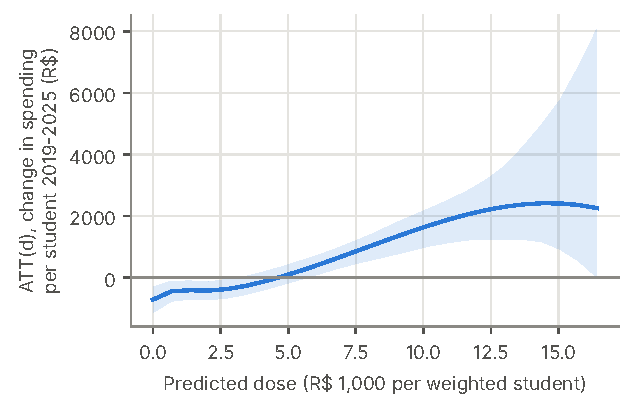
\includegraphics[width=0.55\linewidth]{f5_curva_gasto.pdf}
\caption{Dose-response curve of spending per student, 2019 to 2025. Cubic B-spline with interior knots at the terciles of the positive dose; 95\% bootstrap intervals over immediate regions.}\label{fig:curva}
\end{figure}

\subsection{What the event study shows}

The plan has no event study for spending; Figure~\ref{fig:evento_gasto} adds one, labelled exploratory. Panel a shows that, relative to 2019, spending per student in high-dose networks was higher in every year from 2015 to 2018, by \reais{}~110 to 169 per \reais{}~1,000 of dose, and the pre-trend test rejects ($p=0.001$). In other words, 2019, the base year of the formula, is a trough, a version of the dip before program entry described by \citet{ashenfelter1978}. Measured from 2017 the long difference to 2025 is \reais{}~3 (standard error 24), and measured from the mean of 2015 to 2018 it is $-18$ (24).

Panels b and c separate the numerator from the denominator. Total spending has no differential trend before 2019: the coefficients from 2015 to 2018 lie between $-0.3$ and $+0.1$ log points. Enrollment, in contrast, grew steadily into 2019 and stopped growing after 2020. The trough in spending per student is the denominator: the networks that the formula selects were adding students faster than their spending grew.

\begin{figure}[!htbp]
\centering
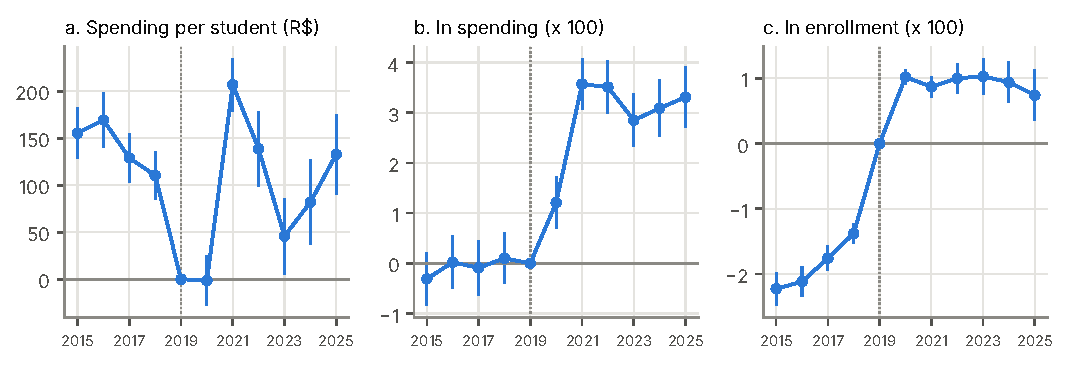
\includegraphics[width=\linewidth]{f3_evento_gasto.pdf}
\caption{Event studies of spending. Coefficients of the dose relative to 2019, with unit and state-by-year fixed effects and the covariates interacted with year; 95\% intervals clustered by immediate region. Exploratory, not in the plan.}\label{fig:evento_gasto}
\end{figure}

\subsection{Where the extra spending came from}\label{sec:fontes}

Figure~\ref{fig:fontes} decomposes total education spending using the revenue lines of the municipal accounts, all divided by the enrollment of 2019, so that the components add up and the enrollment trend stays out of them (exploratory). Education spending on this denominator has no differential trend before 2019 ($p=0.06$) and rises by \reais{}~84 per student per \reais{}~1,000 of dose in 2020, \reais{}~289 in 2021 and \reais{}~252 in 2025.

The VAAT money actually received accounts for about half of the increase. In 2021 it is \reais{}~164 per \reais{}~1,000 of dose, as predicted, and the Union complementation recorded as revenue in the municipal accounts matches it (\reais{}~169). From 2022 on it falls to between \reais{}~96 and \reais{}~131, while the formula predicts \reais{}~224 to \reais{}~314. The networks that the 2021 position ranks highest received less than predicted, because their own VAAT rose after 2021.

The other half matches the transfers from the state-level Fundeb, which each state redistributes among its networks by weighted enrollment. These receipts have no differential trend before 2019 ($p=0.39$), rise by \reais{}~74 per \reais{}~1,000 of dose in 2020, before any VAAT payment, and by \reais{}~147 to \reais{}~168 from 2021 on. They follow the enrollment growth documented in Section~\ref{sec:onde}, and from 2021 the new weights of the reform. Because the VAAT of each year uses the revenues of two years before, these receipts also raise a network's VAAT and lower its complementation two years later, which is consistent with the gap between the predicted and the received VAAT money. The dose therefore measures exposure to two things at once: the VAAT, and the share of the state funds that follows enrollment. The design cannot separate them, and total spending is not the outcome the plan registered.

\begin{figure}[!htbp]
\centering
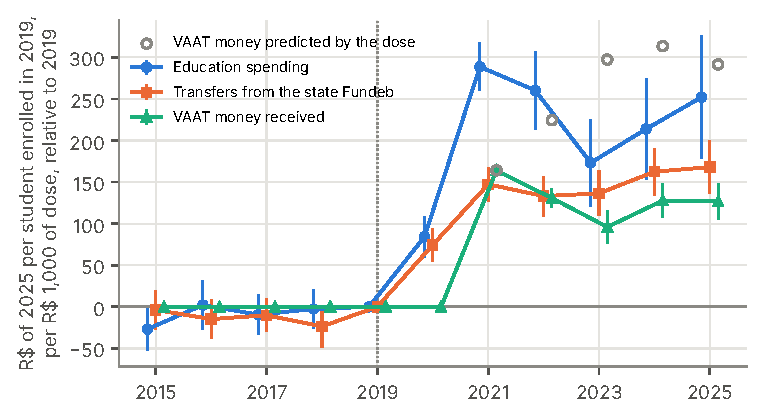
\includegraphics[width=0.75\linewidth]{f9_decomposicao.pdf}
\caption{Where the extra spending came from. Event-study coefficients of the dose, relative to 2019, for education spending and for two revenue lines of the municipal accounts (DCA, Annex I-C), all in reais of 2025 per student enrolled in 2019; specification of Figure~\ref{fig:evento_gasto}. VAAT money received: the December portarias and the 2023 and 2024 adjustments, times the weighted enrollment of the 2021 VAAT. Hollow markers: the VAAT money that the dose predicts. Exploratory, not in the plan.}\label{fig:fontes}
\end{figure}

\subsection{The regression kink}

The kink at the 2021 threshold should identify the pass-through of the first transfers, but the plan's addendum warned that its minimum detectable pass-through is about 3. Table~\ref{tab:kink} confirms that it is uninformative: the estimate is 0.83, with a robust interval from $-6.6$ to 4.6. The validity checks pass: no kink in predetermined variables, no kink at placebo thresholds, and no discontinuity in the density of $x$ ($p=0.50$). Even the data check, the kink in the complementation recorded as revenue, which should be one, has an interval from $-0.4$ to 3.3. The permutation test of \citet{ganong2018} rejects ($p<0.005$), but it implies a pass-through near 3.5, and in simulations on the real support of $x$ it rejects too often under the null (Appendix~\ref{app:sim}); I do not read it as evidence.

\section{School inputs}\label{sec:insumos}

Table~\ref{tab:insumos} reports the 28 pre-registered tests on spending by stage and school inputs. Six pass the Benjamini-Hochberg threshold of 0.05. Spending per student rose with the dose in early childhood, by \reais{}~158 per \reais{}~1,000 in 2025, and in fundamental, by \reais{}~150 in 2025 and \reais{}~223 in 2023. Creche enrollment grew less in high-dose networks, by 3.8 log points per \reais{}~1,000 between 2019 and 2025 and by 4.3 between 2019 and 2023, and the full-time share of fundamental grew less, by 0.7 points by 2025.

\begin{table}[!htbp]
\centering
\caption{Spending by stage and school inputs (S2)}\label{tab:insumos}
\small
\begin{adjustbox}{max width=\linewidth}
\begin{tabular}{lrrrrrr}
\toprule
 & \multicolumn{3}{c}{2019 to 2023} & \multicolumn{3}{c}{2019 to 2025} \\
\cmidrule(lr){2-4}\cmidrule(lr){5-7}
Outcome & $\beta$ & (SE) & $q$ & $\beta$ & (SE) & $q$ \\
\midrule
Spending per student, early childhood (R\$) & 154.7 & (80.6) & 0.156 & 157.9 & (46.4) & 0.007 \\
Spending per student, fundamental (R\$) & 223.2 & (79.6) & 0.032 & 149.6 & (54.0) & 0.032 \\
ln enrollment, creche & $-$0.0427 & (0.0108) & 0.001 & $-$0.0378 & (0.0068) & 0.000 \\
ln enrollment, pre-school & 0.0070 & (0.0029) & 0.053 & 0.0045 & (0.0018) & 0.053 \\
Full-time share, creche & $-$0.0040 & (0.0044) & 0.494 & $-$0.0047 & (0.0027) & 0.213 \\
Full-time share, pre-school & 0.0044 & (0.0048) & 0.494 & $-$0.0044 & (0.0029) & 0.260 \\
Full-time share, fundamental & $-$0.0043 & (0.0045) & 0.494 & $-$0.0070 & (0.0027) & 0.048 \\
Students per class, early grades & $-$0.0590 & (0.0684) & 0.494 & $-$0.0445 & (0.0397) & 0.410 \\
Teachers per 100 students & 0.0275 & (0.0162) & 0.213 & 0.0265 & (0.0115) & 0.068 \\
Teachers with higher education, early childhood (\%) & $-$0.1623 & (0.2550) & 0.586 & 0.1636 & (0.1462) & 0.410 \\
Teachers with higher education, fundamental (\%) & $-$0.2134 & (0.1714) & 0.399 & 0.0114 & (0.1003) & 0.910 \\
Daily hours, creche & $-$0.0131 & (0.0220) & 0.586 & $-$0.0087 & (0.0126) & 0.574 \\
Daily hours, pre-school & 0.0247 & (0.0214) & 0.410 & $-$0.0096 & (0.0124) & 0.536 \\
Daily hours, early grades & 0.0271 & (0.0178) & 0.260 & $-$0.0067 & (0.0116) & 0.586 \\
\bottomrule
\end{tabular}
\end{adjustbox}
\par\smallskip\begin{minipage}{0.95\linewidth}\footnotesize Change from 2019, per R\$ 1,000 of predicted dose (summed up to the outcome year). Specification as in Table 2. $q$: Benjamini-Hochberg over the 28 tests.\end{minipage}

\end{table}

These results inherit the problem of Section~\ref{sec:gasto}: they are changes from 2019 in quantities divided by enrollment or in enrollment itself. The creche result is the clearest case. In the exploratory event study, municipal creche enrollment in high-dose networks grew faster than elsewhere until 2019 and 2020 and slower afterwards (Figure~\ref{fig:matriculas_creche} in Appendix~\ref{app:extra}), so the negative estimate measures the end of an earlier expansion as much as anything the VAAT did, even though half of the money is earmarked for early childhood.

\section{Learning}\label{sec:aprendizagem}

\subsection{The pre-registered estimates}

Table~\ref{tab:aprendizagem} reports the primary learning outcomes. Per \reais{}~1,000 of dose, $N$ rose by 0.0088 points in the 5th grade (Holm-adjusted $p=0.22$) and by 0.0077 in the 9th ($p=0.22$). At the 75th percentile of the dose this is 0.022 student standard deviations in both grades, with 95\% intervals from $-0.005$ to 0.050 and from $-0.011$ to 0.055. $\text{ATT}^o$ is 0.010 standard deviations in the 5th grade and $-0.002$ in the 9th, neither distinguishable from zero. None of the 11 secondary learning outcomes passes the Benjamini-Hochberg threshold; the smallest $q$-value is 0.21. The INSE of the network, a measure of who the students are, did not change with the dose in the pre-registered estimate, although its $\text{ATT}^o$ is negative ($-0.015$, interval $-0.025$ to $-0.005$).

\begin{table}[!htbp]
\centering
\caption{Learning (P2 and S1)}\label{tab:aprendizagem}
\small
\begin{adjustbox}{max width=\linewidth}
\begin{tabular}{lrrrrc}
\toprule
Outcome & $\beta$ & (SE) & Adjusted $p$ & At p75, SD & 95\% interval at p75, SD \\
\midrule
N, 5th grade (P2) & 0.0088 & (0.0055) & 0.219 & 0.022 & [$-$0.005, 0.050] \\
N, 9th grade (P2) & 0.0077 & (0.0058) & 0.219 & 0.022 & [$-$0.011, 0.055] \\
\midrule
Ideb, 5th grade & 0.0080 & (0.0056) & 0.239 &  & \\
Mathematics (points), 5th grade & 0.254 & (0.161) & 0.239 & 0.024 & \\
Portuguese (points), 5th grade & 0.260 & (0.147) & 0.211 & 0.025 & \\
Flow indicator P, 5th grade & $-$0.0002 & (0.0004) & 0.640 &  & \\
Ideb, 9th grade & 0.0019 & (0.0060) & 0.748 &  & \\
Mathematics (points), 9th grade & 0.275 & (0.191) & 0.239 & 0.026 & \\
Portuguese (points), 9th grade & 0.188 & (0.170) & 0.330 & 0.018 & \\
Flow indicator P, 9th grade & $-$0.0011 & (0.0006) & 0.211 &  & \\
N, 2019 to 2023, 5th grade & 0.0173 & (0.0096) & 0.211 & 0.023 & \\
N, 2019 to 2023, 9th grade & 0.0191 & (0.0091) & 0.211 & 0.029 & \\
INSE of the network, 2019 to 2023 & $-$0.0023 & (0.0019) & 0.309 &  & \\
\bottomrule
\end{tabular}
\end{adjustbox}
\par\smallskip\begin{minipage}{0.95\linewidth}\footnotesize Change from 2019 to 2025 unless stated, per R\$ 1,000 of predicted dose. Specification as in Table 2. P2: Holm-adjusted $p$ across the two grades; S1 (below the line): Benjamini-Hochberg $q$ over 11 tests. SD: student standard deviations (one point of N is 0.507 SD in the 5th grade and 0.574 in the 9th; scores use the student SD of public schools in 2023).\end{minipage}

\end{table}

The plan fixed how a null result is reported: by the largest effect the interval does not exclude. At the 75th percentile of the dose, that is 0.050 student standard deviations in the 5th grade and 0.055 in the 9th. The plan's power calculation put the minimum detectable effect at 0.037 and the effect expected under the returns that \citet{jackson2024} estimate for the United States at 0.018. The data therefore rule out large effects, but not effects of the size the international evidence suggests, and the point estimates are close to that size.

The estimates are positive in every robustness check, and significant in three. With the 2019 level as a covariate, which the plan does not prefer because conditioning on the baseline level can itself bias a difference-in-differences when groups differ in levels, they are 0.015 and 0.012. Trimming the tails of the change gives 0.011 in the 5th grade. With the dose from the money actually received they are 0.042 and 0.043; that dose depends on enrollment after 2021, which is exactly why the plan uses the predicted one. In the 5th grade the estimate is larger in the Northeast (0.015 against $-0.010$, $p=0.017$ for the difference, one of six heterogeneity tests).

\subsection{Trends}

The pre-trend tests do not reject: $p=0.39$ in the 5th grade and 0.71 in the 9th. By the rules of the plan as amended, the learning results are not marked as fragile. Figure~\ref{fig:evento_N} shows why they should still be read with care in the 5th grade. The coefficients rise steadily from $-0.015$ in 2005 to $-0.005$ in 2017, zero in 2019 and 0.009 in 2025, close to the line fitted to 2009 to 2017. The joint test has little power against a smooth trend \citep{roth2022}. Net of the trend, the pre-registered sensitivity analysis gives 0.003 per \reais{}~1,000 in the 5th grade (standard error 0.009), or 0.007 standard deviations at the 75th percentile, with an interval from $-0.040$ to 0.055. In the 9th grade there is no such trend, and net of the fitted line the estimate is 0.016 (0.009), or 0.046 standard deviations, with an interval from $-0.002$ to 0.095.

\begin{figure}[!htbp]
\centering
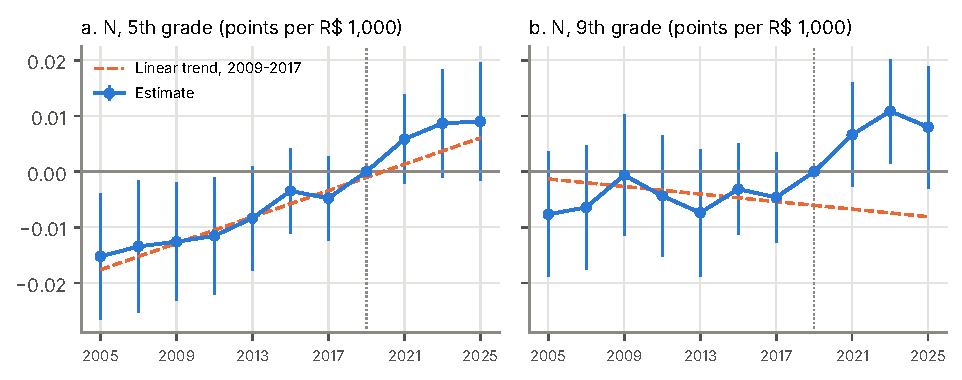
\includegraphics[width=0.95\linewidth]{f6_evento_N.pdf}
\caption{Event studies of $N$, the standardized Saeb mean of the municipal network. Coefficients of the dose relative to 2019 with 95\% intervals; dashed line: linear trend fitted to the coefficients of 2009 to 2017 and extrapolated, as pre-registered. The 2021 coefficient is reported but not interpreted (pandemic round).}\label{fig:evento_N}
\end{figure}

The relative-magnitudes bounds do not help much in this design. The original interval for 2025 already includes zero in both grades, so the breakdown value of $\bar M$ is zero; with $\bar M=1$ the interval spans $-0.028$ to 0.043 per \reais{}~1,000 in the 5th grade and $-0.032$ to 0.048 in the 9th. As the simulations behind the addendum showed, with 2025 three rounds after the reference year these bounds are wide even when trends are exactly parallel.

\subsection{Within municipalities}

Table~\ref{tab:dentro} compares the municipal and the state network of the same municipality, in the 816 municipalities with both networks observed in the 5th grade and the 1,081 in the 9th. The difference is $-0.031$ standard deviations at the 75th percentile in the 5th grade and 0.000 in the 9th, with intervals that reach $-0.106$ and 0.045, and $-0.069$ and 0.070. The negative control, the state network alone, is close to zero in both grades. The comparison absorbs local shocks, but it is exposed to the movement of students between the two networks documented in Section~\ref{sec:onde}, which changes the composition of both, and a non-significant negative control is weak evidence: in simulations it detected a confounder that biased the main estimate by 22\% only 8\% of the time.

\begin{table}[!htbp]
\centering
\caption{Within-municipality comparison and negative control}\label{tab:dentro}
\small
\begin{adjustbox}{max width=\linewidth}
\begin{tabular}{lrrrcr}
\toprule
Outcome & $\beta$ & (SE) & At p75, SD & 95\% interval & Municipalities \\
\midrule
Municipal network, same municipalities, 5th grade & $-$0.0032 & (0.0125) & $-$0.008 & [$-$0.071, 0.054] & 816 \\
Within municipality (municipal minus state), 5th grade & $-$0.0120 & (0.0150) & $-$0.031 & [$-$0.106, 0.045] & 816 \\
Negative control: state network, 5th grade & 0.0088 & (0.0133) & 0.022 & [$-$0.044, 0.089] & 816 \\
Municipal network, same municipalities, 9th grade & $-$0.0035 & (0.0095) & $-$0.010 & [$-$0.064, 0.043] & 1081 \\
Within municipality (municipal minus state), 9th grade & 0.0002 & (0.0122) & 0.001 & [$-$0.069, 0.070] & 1081 \\
Negative control: state network, 9th grade & $-$0.0037 & (0.0078) & $-$0.011 & [$-$0.055, 0.033] & 1081 \\
\bottomrule
\end{tabular}
\end{adjustbox}
\par\smallskip\begin{minipage}{0.95\linewidth}\footnotesize Change in N from 2019 to 2025, municipalities where both the municipal and the state network have N in 2019 and 2025. Specification as in Table 2.\end{minipage}

\end{table}

Figure~\ref{fig:aprendizagem} brings the learning estimates together. All of them are within a band of about $\pm 0.1$ standard deviations at the 75th percentile of the dose, and none excludes zero.

\begin{figure}[!htbp]
\centering
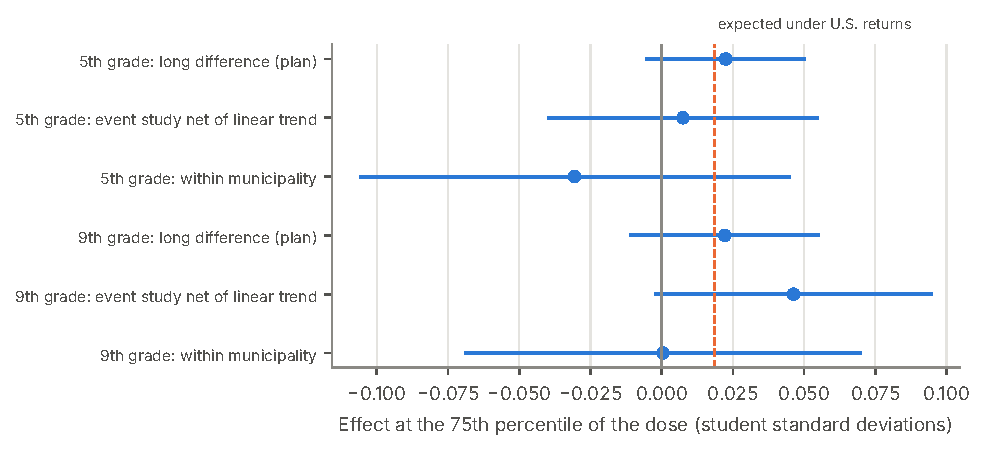
\includegraphics[width=0.8\linewidth]{f7_aprendizagem.pdf}
\caption{Learning estimates at the 75th percentile of the dose, in student standard deviations, with 95\% intervals. Dashed line: effect expected under the returns estimated for the United States \citep{jackson2024}, from the plan's power calculation.}\label{fig:aprendizagem}
\end{figure}

\section{Discussion}\label{sec:discussao}

The VAAT sends federal money to the networks with the least resources per student, and it reached them: they are poorer, in the Northeast, and spent less. The difficulty for evaluation is that the same formula that targets them also selects networks that were changing. Dividing a base-year capacity by base-year enrollment picks networks whose enrollment had been growing, in large part because state schools were being transferred to them. That selection explains why the pre-registered estimate for spending per student is positive while the same comparison, anchored a few years earlier, is zero. It is a lesson for any evaluation of a per-student formula: the denominator of the formula is also the denominator of the outcome.

Total spending, which is not divided by enrollment and shows no differential trend before 2019, rose in high-dose networks by about twice the VAAT money they received. The other half matches the transfers from the state Fundeb, which follow enrollment and rose from 2020, before the VAAT paid anything. The two sources together are somewhat larger than the increase in spending, so the data leave no room for a clean estimate of how much of the VAAT itself was spent. Partial pass-through is common for intergovernmental grants \citep{hines1995,gordon2004}; here the difficulty comes first, because the transfer is not the only money that the dose measures.

On learning, the design is informative about large effects and not about small ones. Effects above about 0.05 standard deviations at the 75th percentile of the dose are unlikely; effects of 0.02, the size implied by the U.S. evidence, are well inside every interval. Two features of the program make large effects unlikely in any case. Half of the money is earmarked for early childhood, which the cohorts tested up to 2025 did not attend under the program. And less money arrived than the formula predicts from 2019 data: summed over 2021 to 2025, the VAAT money received per enrolled student was \reais{}~575 for each \reais{}~1,000 of dose, against \reais{}~1,246 predicted. The plan's expected effect of 0.018 standard deviations was computed from the predicted dose; with the money that arrived, the same returns would imply about 0.008.

The analysis has limits that the data do not allow me to remove. The Saeb participation rate, a check on selection into the test, cannot be linked to municipalities in the public files; the school-level days without in-person classes in 2020 are not public; both were requested from Inep. The Saeb 2025 school files had not been released. And the enrollment shifts between networks that make the design hard are also a possible channel through which the VAAT itself works, which the data cannot separate either.

\section{Conclusion}\label{sec:conclusao}

Brazil's VAAT complementation reached the municipal networks it was designed for. Their spending rose, by about twice the VAAT money they received, together with transfers from the state Fundeb that follow enrollment, and their students' test scores did not change by more than about 0.05 standard deviations at the 75th percentile of exposure. The pre-registered estimate for spending per student is positive, but it reflects the growth in enrollment that the formula itself rewards; in the 5th grade, the positive learning estimate is the continuation of an older trend. The VAAT will keep growing until 2026. Measuring its effects better will require either outcomes that the formula does not divide, or variation in the money that does not come from the networks' own enrollment.


\section*{Data and code availability}
All data are public. The code, the intermediate results and the instructions to reproduce every table and figure are maintained at \url{https://github.com/Caioalexnes/Brazilian-Basic-Education-Analysis}. The scripts download each public file from its original address, and the repository lists the source of every file and the SHA-256 checksums of the downloaded files. The pre-analysis plan and its addendum are archived on Zenodo (\url{https://doi.org/10.5281/zenodo.24391651} and \url{https://doi.org/10.5281/zenodo.24394910}); the dated files that fixed the implementation details before each stage of the analysis are in the repository.
\todo{Archive the submitted version of the repository on Zenodo and add its DOI here and in the title footnote.}

\section*{Declaration of generative AI use}
The author used Claude (Anthropic) throughout this work. The research question originates in an essay by the author on public spending in health and education (in preparation), whose section on basic education related spending to the Ideb. Under the author's direction, the AI system wrote and ran the analysis code in Python and R, produced the tables and figures from that code, searched for and summarized sources, proposed analyses, including the simulations used to test the estimators, and drafted the text of the pre-analysis plan, its addendum and this paper. The author chose the analyses to run and report, approved the pre-analysis plan and each amendment before the corresponding outcomes were used, decided how the results are interpreted, reviewed the results and the sources, and revised the text. The author takes full responsibility for the content. All figures are charts drawn by code from public data; no image was generated or altered by AI. The AI system is not an author.

\section*{Competing interests}
The author reports no competing interests.

\bibliographystyle{plainnat}
\bibliography{refs}

\processdelayedfloats
\clearpage
\section*{Online appendix}
\addcontentsline{toc}{section}{Online appendix}

This appendix, intended for online publication, lists the departures from the pre-analysis plan, documents the data and the conversion of test scores into student standard deviations, summarizes the simulations behind the plan's addendum, and reports the additional results cited in the text.

\appendix
\section{Departures from the plan}\label{app:desvios}

\begin{enumerate}[label=A\arabic*.]
\item \textbf{Addendum 1} (deposited before any outcome was used): wild bootstrap $p$-value for the pre-trend test; breakdown value of $\bar M$ removed from the interpretation rules; note on the negative control; errata on the 2022 share of recipients (37.7\%, not 37.6\%), on the power of the kink (minimum detectable pass-through about 3, not 0.82) and on the software \citep{cunha2026add}.
\item \textbf{Implementation details} of stages 3 and 4, fixed in dated files before the corresponding outcomes were related to the dose (files detalhes\_etapa3.md and detalhes\_etapa4.md in the folder pap of \citealp{cunha2026a}).
\item \textbf{Saeb participation removed from S1.} Inep's public Saeb school files mask the municipality and school codes. My script first aggregated them as if the masked code were the IBGE code; I found the error before any learning outcome was used, corrected the script and removed the outcome. The data were requested from Inep.
\item \textbf{Days without in-person classes in 2020} (robustness check 2) are not public; requested from Inep, protocol 23546.158945/2026-03.
\item \textbf{Saeb 2025 school files} were not released, so the post-treatment round for participation would have been 2023, as the plan provides.
\item \textbf{Analyses not in the plan}, reported as exploratory: the event studies of spending, ln spending and ln enrollment, the benchmarks of predicted and received VAAT money, the long differences from earlier baselines (Figure~\ref{fig:evento_gasto}), the decomposition of spending by revenue source (Figure~\ref{fig:fontes}), and the event studies of enrollment by network (Figure~\ref{fig:matriculas}).
\item \textbf{IPCA series}: extended back to January 2015 to deflate spending in 2015 and 2016; the months already in the repository are unchanged.
\end{enumerate}

\section{Data}\label{app:dados}

$N$ is the mean of mathematics and Portuguese, each rescaled as $10(S - S_{\inf})/(S_{\sup} - S_{\inf})$ with Inep's limits (5th grade: mathematics 60 to 322, Portuguese 49 to 324; 9th grade: 100 to 400). If the effect is $d$ student standard deviations in both subjects, the change in $N$ is $5d(\sigma_{\text{mat}}/r_{\text{mat}} + \sigma_{\text{por}}/r_{\text{por}})$; with the student standard deviations of public schools in the Saeb 2023 (53.4 and 52.4 in the 5th grade, 53.1 and 51.5 in the 9th), one point of $N$ is 0.507 standard deviations in the 5th grade and 0.574 in the 9th. Spending follows the definition of \citet{cunha2026a}: function 12 plus subfunction 847 recorded outside it, minus higher education (subfunction 364). Every number in the text comes from a results file of the repository; the scripts are listed in its README.

\section{Simulations}\label{app:sim}

Script \texttt{21\_teste\_simulado.py} keeps the real dose, state, region, VAAT position and 2021 transfer of the 5,208 networks and simulates covariates and outcomes with known effects. Table~1 of the addendum reports bias, coverage and rejection rates for every estimator. In short: the long difference, the dose-response estimators and the event study are unbiased with coverage between 93\% and 96\%; the cluster-robust pre-trend test over-rejects (8.6\%), the wild bootstrap does not (6.6\%); the breakdown value of $\bar M$ is below 1 in every draw with parallel trends; the negative control detects a confounder that biases the main estimate by 22\% in 8\% of the draws; and the kink is unbiased but has power of 16\% against full pass-through. The permutation test of the kink rejects 6\% to 9\% of the time under the null, because the support of $x$ around the threshold leaves placebo thresholds only between about 0.25 and 0.44, whose estimates overlap.

\section{Additional results}\label{app:extra}
\setcounter{table}{0}\setcounter{posttable}{0}\setcounter{figure}{0}\setcounter{postfigure}{0}
\renewcommand{\thetable}{D\arabic{table}}\renewcommand{\theposttable}{D\arabic{posttable}}\renewcommand{\theHtable}{D\arabic{table}}
\renewcommand{\thefigure}{D\arabic{figure}}\renewcommand{\thepostfigure}{D\arabic{postfigure}}\renewcommand{\theHfigure}{D\arabic{figure}}

\begin{table}[!htbp]
\centering
\caption{Regression kink of spending at the 2021 threshold}\label{tab:kink}
\small
\begin{adjustbox}{max width=\linewidth}
\begin{tabular}{lrcr}
\toprule
Test & Estimate & Robust 95\% interval & $p$ \\
\midrule
Pass-through, main (MSE-optimal h, local linear) & 0.83 & [$-$6.60, 4.57] & 0.722 \\
Pass-through, local quadratic & $-$1.39 & [$-$10.42, 4.27] & 0.411 \\
Pass-through, h = 0.1 & 2.59 & [$-$8.00, 4.25] & 0.549 \\
Pass-through, h = 0.2 & 3.49 & [$-$0.45, 4.55] & 0.108 \\
Data check: complementation recorded as revenue in 2021 & 1.22 & [$-$0.39, 3.34] & 0.121 \\
Difference in kinks: pre-period change (2016-17 to 2018-19) & 1.14 & [$-$0.99, 3.88] & 0.245 \\
Difference in kinks: main minus pre-period change & 0.05 & [$-$9.42, 4.74] & 0.517 \\
Predetermined: 2019 spending per student (reais of 2021) & $-$6{,}680.51 & [$-$50{,}734.23, 25{,}080.73] & 0.507 \\
Predetermined: INSE 2019 & $-$2.79 & [$-$14.34, 4.49] & 0.305 \\
Predetermined: ln population 2020 & $-$2.61 & [$-$23.93, 13.66] & 0.592 \\
Predetermined: ICMS share 2019 & $-$0.61 & [$-$2.62, 0.65] & 0.239 \\
Placebo threshold x = -0.10 & $-$12{,}669.86 & [$-$85{,}596.34, 48{,}236.52] & 0.584 \\
Placebo threshold x = -0.05 & 57{,}742.41 & [$-$137{,}881.42, 309{,}348.18] & 0.452 \\
Placebo threshold x = +0.05 & 8{,}407.49 & [$-$83{,}357.04, 121{,}350.82] & 0.716 \\
Placebo threshold x = +0.10 & 101{,}986.84 & [$-$114{,}920.50, 434{,}035.24] & 0.255 \\
Permutation test (h = 0.2, 200 placebo thresholds) & 20{,}967.74 &  & 0.000 \\
Density test at x = 0 &  &  & 0.505 \\
\bottomrule
\end{tabular}
\end{adjustbox}
\par\smallskip\begin{minipage}{0.95\linewidth}\footnotesize Fuzzy regression kink at the 2021 threshold (\texttt{rdrobust}, local linear, triangular kernel, MSE-optimal bandwidth unless stated). Outcome: change in education spending per enrolled student between 2018-2019 and 2021-2022, reais of 2021. Pass-through: reais of spending per real of 2021 complementation. Sharp kinks for predetermined variables and placebo thresholds.\end{minipage}

\end{table}

\begin{figure}[!htbp]
\centering
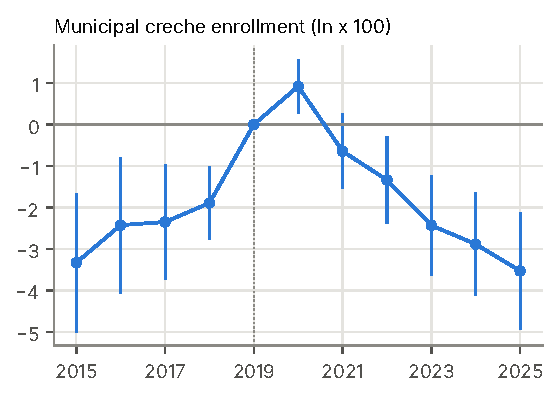
\includegraphics[width=0.55\linewidth]{f8_creche.pdf}
\caption{Municipal creche enrollment. Event-study coefficients of the dose on ln(1 + enrollment), $\times 100$, relative to 2019; specification of Figure~\ref{fig:matriculas}. Exploratory.}\label{fig:matriculas_creche}
\end{figure}

\end{document}
